\chapter{ArcMap Interface}
\section{Objectives of the exercise}
Make trainees familiar with the basic tools in ArcGIS intended to make trainees competent in exploring the data.

\section{Data Information}
You will use the following data.
\begin{enumerate}
\item{LocalUnits | Local Units of Nepal | Polygon data}
\item{DIS\textunderscore HQ | District Headquarter | Point data}
\item{MajorRivers | Major Rivers of Nepal | Line data}
\item{Districts | District Boundary | Polygon Data}
\item{RoadNetwork2006 | Road Network | Line data}
\end{enumerate}

\section{Steps}
\subsection{Opening ArcMap 10.5}
\begin{enumerate}
\item{Start |  ArcGIS  | ArcMap 10.5}
\item{You will see the window as shown in figure \ref{fig:ArcMap_Interface}.}
	\begin{figure}[h]
	\label{fig:ArcMap_Interface}
	\centering
	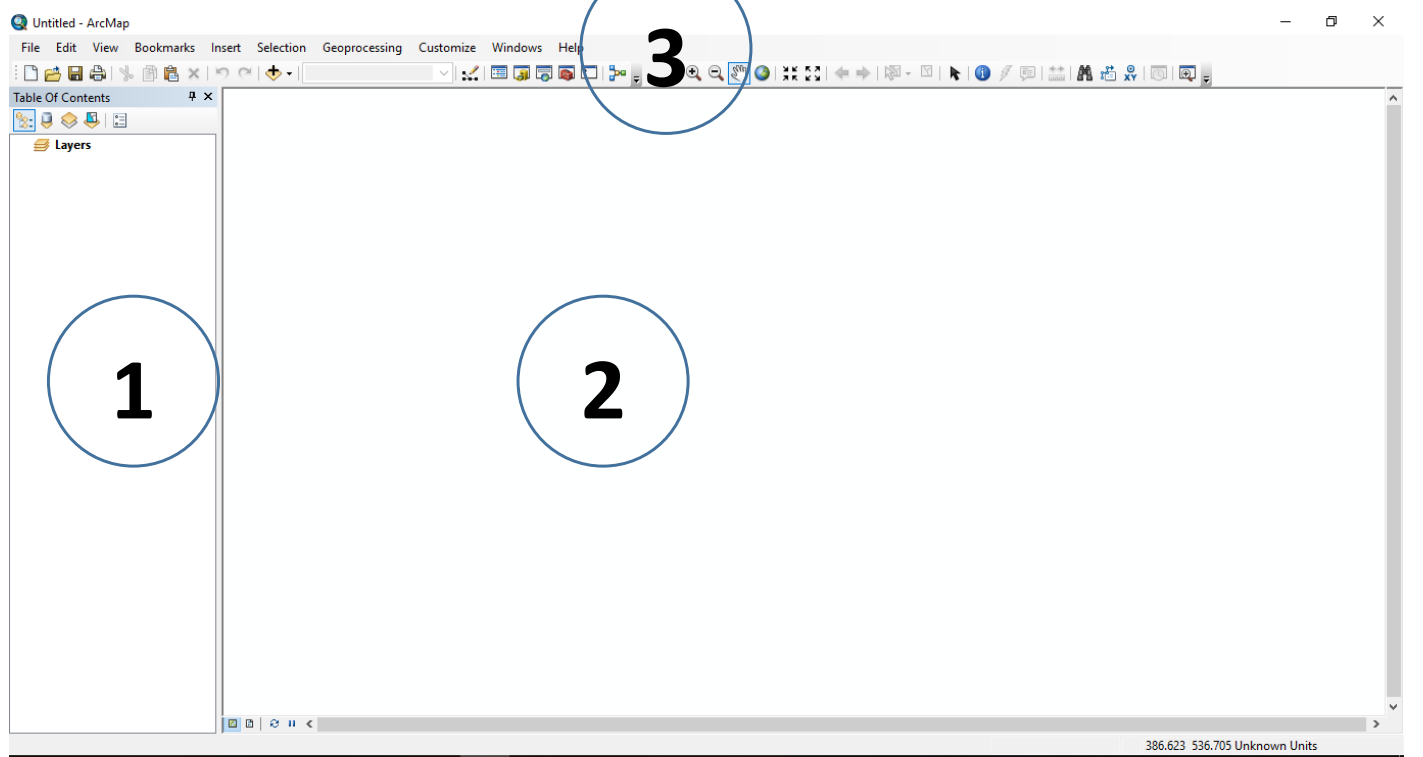
\includegraphics[scale=0.5]{images/interface}
	\caption{ArcMap Interface}
	\end{figure}
\item{On the left side, you see Table of Contents(1).}
\item{The large white part is the Map Canvas (2)}
\item{On the upper part you see several toolbars (3)}
\item{Among the toolbars, there is a standard toolbar as shown in figure \ref{fig:Standard_Toolbar}}
	\begin{figure}[h]
	\label{fig:Standard_Toolbar}
	\centering
	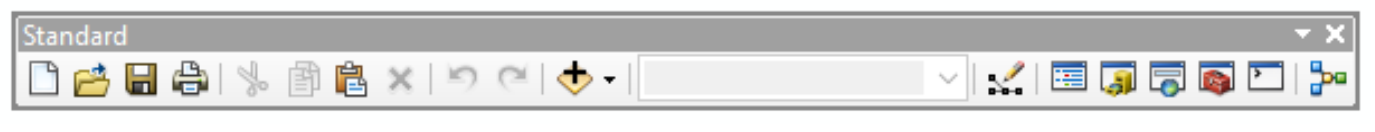
\includegraphics[scale=0.5]{images/standard_toolbar}
	\caption{Standard Toolbar}
	\end{figure}
\item{Hover the mouse over each tool in the toolbar and note their functions.}
\end{enumerate}

\subsection{Adding Data}
\begin{enumerate}
\item{Click on the Add Data icon on standard toolbar.}
\item{Browse to the data folder and add Districts data.}
\item{Districts is a vector data in shapefile (.shp) format.}
\item{You will see the data displayed on the Map Canvas as well as the Districts layer in the table of contents.}
\item{Each geographical (spatial) data also have attribute information and so does the Districts layer.}
\item{Right click on the Districts layer in \emph{Table of contents} and click Open Attribute Table.}
\item{Note the attributes.}
\item{Tip 1 : You can sort (ascending/descending) any attribute values by double clicking each attribute name.}
\item{Tip 2 : You can see the total number of data at the bottom of the attribute table}
\item{Close the attribute table}
\end{enumerate}

\subsection{Basic Navigation Tools}
\begin{enumerate}
\item{Among the toolbars, there is a toolbar called Tools as shown in figure.}
\begin{figure}[h]
	\label{fig:Tool_Toolbar}
	\centering
	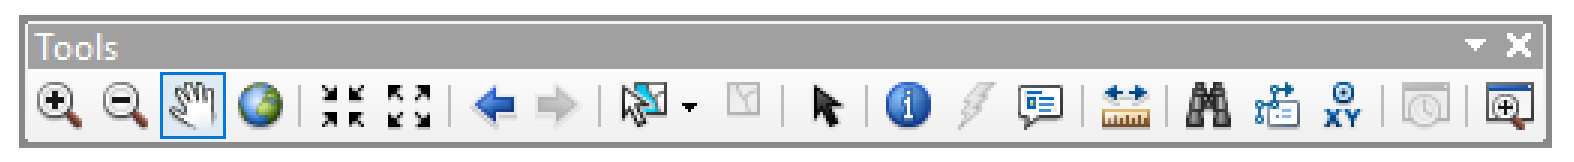
\includegraphics[scale=0.5]{images/tool_toolbar}
	\caption{Tool Toolbar}
	\end{figure}
\item{Hover the mouse over each tools and note the names.}
\item{Now use each of the tools to navigate through the maps. There are tools for zoom, pan, full, extent, etc.}
\end{enumerate}

\subsection{Queries for practice}
Explore various tools to determine the following:
\begin{enumerate}
	\item{Find the area of the largest and smallest district of Nepal.}
	\item{What is the area of Nepal?}
\end{enumerate}

\subsection{Adding additional data}
Add all the remaining data.
\begin{enumerate}
	\item{Rearrange the layers by dragging the layers in \emph{Table of Contents} to place it one over another in the order that you want.}
	\item{Check/uncheck the layers in the \emph{Table of Contents} to display or not to display individual layers.}
	\item{For each layer, note the attributes.}
\end{enumerate}

\subsection{Additional practice queries}
\begin{enumerate}
	\item{What is the total number of local units?}
	\item{What is the area of your district?}
	\item{What is the distance between Kathmandu and Dharan?}
	\item{If you have to walk around a district along it's boundary, which district would offer you the longest walk?}
	\item{What is the perimeter of Nepal?}
\end{enumerate}









